\documentclass[conference]{IEEEtran}
\usepackage{xcolor}
\usepackage{url}
\usepackage{graphicx} 
\usepackage{amssymb}
\usepackage{amsmath}
\usepackage{algpseudocode}
\usepackage{algorithm}
\usepackage{listings}
\usepackage{tikz}
\usetikzlibrary{positioning, fit}
\usepackage{xcolor}
\usepackage[colorlinks=true,linkcolor=blue,citecolor=blue,urlcolor=blue]{hyperref}
\usepackage{tikz}
\usetikzlibrary{shapes.geometric, arrows}
\algrenewcommand\algorithmicrequire{\textbf{Input:}}
\algrenewcommand\algorithmicensure{\textbf{Output:}}

\definecolor{codegreen}{rgb}{0,0.6,0}
\definecolor{codegray}{rgb}{0.5,0.5,0.5}
\definecolor{codepurple}{rgb}{0.58,0,0.82}
\definecolor{backcolour}{rgb}{0.97,0.97,0.97}

\lstdefinestyle{mypython}{
    backgroundcolor=\color{backcolour},   
    commentstyle=\color{codegreen},
    keywordstyle=\color{blue}\bfseries,
    numberstyle=\tiny\color{codegray},
    stringstyle=\color{codepurple},
    basicstyle=\ttfamily\footnotesize,
    breakatwhitespace=false,         
    breaklines=true,                 
    captionpos=b,
    keepspaces=true,                 
    numbers=left,                    
    numbersep=5pt,                  
    showspaces=false,                
    showstringspaces=false,
    showtabs=false,                  
    tabsize=4,
    language=Python
}

\hyphenation{op-tical net-works semi-conduc-tor}
\definecolor{uf_blue}{RGB}{17,27, 150}
\definecolor{uf_orange}{RGB}{150,100,17}

\begin{document}

\title{GatorPy: A Custom Implemented Linear Programming Solver}

\author{
    \begin{minipage}{0.50\textwidth}
        \centering
        \textcolor{uf_blue}{Andrés Espinosa} \\
        \textcolor{uf_orange}{Industrial and Systems Engineering} \\
        \textcolor{uf_orange}{University of Florida} \\
        \textcolor{uf_orange}{andresespinosa@ufl.edu} \\ 
    \end{minipage}
}


\maketitle


\begin{abstract}
GatorPy is a pedagogically motivated Linear Programming (LP) solver implemented in pure Python and NumPy. 
The project aims to demystify the internal workings of LP solvers by providing a modular, object-oriented framework that transforms symbolic problem descriptions into slack form and solves them using the two-phase Simplex method. 
The solver supports a custom modeling language and is designed to be readable, extensible, and transparent for students and practitioners embarking on similar projects. 

GatorPy has been validated against CVXPY on a suite of small LPs, successfully passing 6 out of 7 tests. 
The remaining failure highlights the solver's current limitations in handling auxiliary variable removal, motivating iterative improvements as an open-source UF solver. 
There are several directions for continued development of GatorPy, including a more robust test suite, performance-oriented reimplementation in a compiled language, and support for mixed-integer programs, convex programs, alternative solver algorithm. 
GatorPy offers both a functional LP solver and an exciting opportunity as an open-source educational platform for understanding computational optimization fundamentals.    
\end{abstract}

\IEEEpeerreviewmaketitle

\section{Introduction}
\label{sse:introduction}
GatorPy is a custom Linear Programming (LP) solver implemented entirely in Python. 
It is built using native Python constructs and NumPy for numerical operations, and follows an object-oriented programming (OOP) approach to ensure modularity and extensibility. 
GatorPy transforms user-defined LP problems into a structured internal representation, reduces the problem to an equivalent standard form, and applies established solving algorithms to compute optimal solutions.
This project report outlines the implementation of GatorPy and its modular design, which enables future enhancements to the solver. 

The remainder of the introduction, Section~\ref{sse:introduction}, provides an overview of linear programming, the simplex algorithm, existing Operations Research (OR) solvers, and the motivation behind developing GatorPy. 
The implementation is discussed in detail in Section~\ref{sse:implementation}, highlighting key design choices made throughout the development process. 
The section begins with an overview of GatorPy's intuitive modeling syntax, followed by an explanation of the simplex algorithm in pseudocode. 
Next, the core Python objects that serve as the backbone of the framework are introduced. 
Finally, the internal transformations that convert a user-defined GatorPy problem into a solvable slack form LP are described.
Section~\ref{sse:results} presents the testing suite used to validate the functionality of the project, along with instructions on how to deploy and run GatorPy.
The conclusion, Section~\ref{sse:discussion}, outlines potential directions for future work and concludes this report.

\subsection{Linear Programming}

Linear Programming (LP) is a mathematical optimization technique for achieving the best outcome in a mathematical model whose requirements are represented by linear relationships. 
LP has vast applications across various fields, including economics, supply chain, chemical engineering, and industrial engineering. 
An LP problem typically involves an objective function, which is to be maximized or minimized, subject to a set of linear constraints.

Formally, an LP problem can be expressed as:
\[
\text{minimize} \quad \mathbf{c}^\top \mathbf{x}
\]
subject to:
\[
\mathbf{A} \mathbf{x} \preceq \mathbf{b}
\]
where:
\begin{itemize}
    \item \(\mathbf{x} \in \mathbb{R}^n\) is the vector of decision variables,
    \item \(\mathbf{c} \in \mathbb{R}^n\) is the vector of coefficients of the objective function,
    \item \(\mathbf{A} \in \mathbb{R}^{m \times n}\) is the matrix of coefficients of the constraints,
    \item \(\mathbf{b} \in \mathbb{R}^m\) is the right-hand side vector of the constraints.
\end{itemize}


LP problems are highly versatile and many problems that are naturally found across domains can be identically turned into an LP or approximated as one.
The goal of an LP solver is to find the values of \(\mathbf{x}\) that maximize or minimize the objective function while satisfying all the constraints.

\subsection{Simplex Algorithm}

The Simplex algorithm is one of the most widely used methods for solving linear programming problems. 
It is an iterative method that navigates along the edges of the feasible region (defined by the constraints) to reach the optimal solution. 
The algorithm was developed by George Dantzig in 1947 and has since become a cornerstone of operational research and optimization.

The key advantages of the Simplex algorithm include its ability to efficiently handle large problems and its ability to identify both optimal solutions and infeasibility/unboundedness in the problem. 
However, the algorithm's worst-case performance can be exponential in the number of variables, although in practice, it often performs very well.
The Simplex algorithm is also remarkably simple and intuitive, as it works by traversing the corner points of a polyhedron until it lands on the smallest objective-valued corner point.
This concept is shown visually \cite{img:simplex} in Image~\ref{fig:simplex}.

\begin{figure}[htbp]
  \centerline{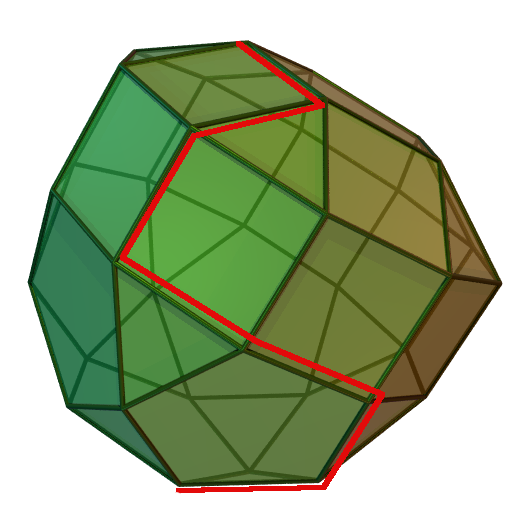
\includegraphics[width=0.25\textwidth]{images/simplex.png}}
  \caption{Visual interpretation of the Simplex traversal}
  \label{fig:simplex}
\end{figure}

Several variants of the Simplex algorithm exist, including primal, dual, and revised forms. 
In GatorPy, the algorithm is implemented using the two-phase Simplex method, which allows the solver to systematically handle LPs with or without an initially feasible solution. 
This approach ensures the user can input any LP in the expected modeling language and solver will handle feasibility, detect unboundedness, and return optimal solutions when they exist.

\subsection{Available Solvers}

There are numerous optimization solvers available, both commercial and open-source, that implement LP solvers and other optimization methods. 
Some of the most popular commercial solvers include:
\begin{itemize}
    \item \textbf{CPLEX}: A high-performance commercial optimization solver by IBM that provides a robust set of optimization algorithms, including the Simplex method and interior-point methods.
    \item \textbf{Gurobi}: Another leading commercial optimization solver, known for its speed and reliability, and used in a wide range of industries.
    \item \textbf{Excel Solver}: A built-in optimization tool in Microsoft Excel that allows users to solve LP problems directly within a spreadsheet interface. 
\end{itemize}

In the open-source domain, several solvers offer accessible alternatives to commercial solutions:
\begin{itemize}
    \item \textbf{GLPK (GNU Linear Programming Kit)}: A popular open-source LP solver that implements both the Simplex method and interior-point methods.
    \item \textbf{COIN-OR}: A collection of open-source optimization solvers, which includes Clp (the COIN-OR LP solver).
    \item \textbf{CVXPY}: A Python-based optimization modeling language that provides a high-level interface for solving LP and convex optimization problems. 
    CVXPY allows for easy integration of different solvers and has become a widely adopted tool in academic and industrial settings.
\end{itemize}

GatorPy is primarily inspired by CVXPY, with a strong emphasis on educational value and extensibility. 
Solvers can often be quite complex due to the advanced techniques they use to optimize computation time. 
By building a custom solver in Python, GatorPy offers greater transparency and customization, making it an ideal tool for students to better understand the underlying principles.



\subsection{Motivation}
The "behind-the-scenes" complexity of solvers often leads students to lose sight of the overall goals and concepts of OR. Many students need an intuitive understanding of the tools they use in order to truly connect with the material. 
This project has two main objectives: First, to provide an educational tool by offering a clear and simple implementation of a linear programming (LP) solver, built entirely using Python and NumPy. 
Second, to lay the groundwork for an open-source solver that can be further developed by future UF students, offering an opportunity for students to engage directly with the core concepts of LP solving.
\section{Implementation}
\label{sse:implementation}
The implementation of GatorPy can be divided into four key parts:

\begin{enumerate}
    \item \textbf{Algebraic Modeling Language}: The first part involves the creation of a custom algebraic modeling language for GatorPy. 
    This syntax is designed to strike a balance between pythonic pseudo-code and an algebraic language interface, making it intuitive for formulating linear programming problems. 
    Further details on its implementation can be found in Section~\ref{Syntax}.
    
    \item \textbf{Simplex Algorithm}: The second part covers the implementation of the Simplex algorithm. 
    This algorithm takes a linear programming problem in slack form and outputs the optimal solution, or an infeasibility/unboundedness certificate if applicable. 
    A detailed explanation of the Simplex algorithm implementation is available in Section~\ref{Simplex}.
    
    \item \textbf{Python Objects}: The third part involves the development of Python objects to support the GatorPy modeling language. 
    These objects are designed to streamline the modeling process and facilitate problem-solving. 
    Their purpose and design are discussed in Section~\ref{Objects}.
    
    \item \textbf{Reductions for Slack Form}: A significant portion of this project focuses on a series of reductions that transform any given LP problem into an equivalent form that can be processed by the Simplex algorithm. 
    This transformation process is integral to the solver's functionality.
\end{enumerate}
\subsection{GatorPy Syntax}
\label{Syntax}
GatorPy makes extensive use of the NumPy numerical processing package, ensuring high performance while using the infamously slow language of Python. 
To effectively model linear programming problems, GatorPy relies on a set of key user-inputted objects that structure the problem.
The structure of a typical GatorPy problem involves the following steps:

\begin{enumerate}
    \item Create \texttt{Parameter} objects for each parameter in the problem.
    Each \texttt{Parameter} object takes in a \texttt{np.array} as the value.
    \item Create \texttt{Variable} objects for each variable in the problem.
    Each \texttt{Variable} takes in an integer as the shape of the vector.
    \textit{Note: Each variable must be a vector, this is left as a potential next step in section \ref{future_work}}.
    \item Create a \texttt{Problem} object representing the overall problem.
    The \texttt{Problem} object expects a Python \texttt{dict} object with the following key-value pairs:
    \begin{itemize}
        \item Either \texttt{"minimize"} or \texttt{"maximize"} as a key with a GatorPy \texttt{Expression} as the value.
        \item Either \texttt{"subject to"} or \texttt{"constraints"} as a key with a list of GatorPy \texttt{Constraint} objects as the value.
    \end{itemize}
\end{enumerate}
The primary objective of GatorPy's optimization modeling syntax is to balance a pythonic interface with standard linear algebraic notation.
The simple syntax of GatorPy can be best communicated with an example.
Consider the following optimization problem with two variables and three constraints:
\begin{align*}
  \text{maximize} & \quad \textbf{c}^\top \textbf{y} \\
  \text{subject to} & \quad \textbf{A} \textbf{y} \preceq \textbf{b} \\
  & \quad \textbf{y} \preceq \textbf{1} \\
  & \quad \textbf{y} \succeq \textbf{0}
\end{align*}
where
\begin{align*}
    \textbf{c} = \begin{bmatrix} 1.2 \\ 0.5 \end{bmatrix}, \quad
    \textbf{A} = \begin{bmatrix} 1 & 1 \\ 1.2 & 0.5 \end{bmatrix}, \quad
    \textbf{b} = \begin{bmatrix} 1 \\ 1 \end{bmatrix}, \quad
    \textbf{y} = \begin{bmatrix} y_1 \\ y_2  \end{bmatrix}
\end{align*}

This above optimization problem can be expressed in GatorPy as:
\begin{lstlisting}[style=mypython, caption={Solving a Linear Program Symbolically}]
# Parameters
A = Parameter(np.array([[1,1],[1.2,0.5]]))
b = Parameter(np.array([1,1]))
c = Parameter(np.array([1.2,1]))

# Variables
y = Variable(2)

# Problem
problem = Problem({
    'maximize': c.T @ y,
    'subject to': [
        A @ y <= b,
        y <= 1,
        y >= 0
    ]
})

solution = problem.solve()
print(solution)
>>> (1.14, [0.71, 0.29], True)
\end{lstlisting}

\subsection{Simplex Implementation}
\label{Simplex}
The implementation of the Simplex algorithm in GatorPy uses  the two-phase simplex method, which will solve for optimality without needing to explicitly enter a feasible starting point.
This version of the simplex algorithm is divided into two main phases: an initial feasibility search phase (Phase 1), and an optimality algorithm (Phase 2). 
A high-level pseudo-code of the two-phase simplex algorithm is available in Algorithm \ref{alg:two_phase_simplex}, while the individual algorithm pseudocodes are located in the Appendix in section \ref{appendix}.


\subsubsection{Phase 1: Finding a Feasible Solution}
The goal of Phase 1 is to find a basic feasible solution (BFS) for the given linear programming problem. If the problem is infeasible, Phase 1 will detect this and terminate. The process involves:
\begin{enumerate}
    \item Augmenting the constraint matrix \( A \) with artificial variables to form an auxiliary problem.
    \item Minimizing the sum of the artificial variables to determine feasibility.
    \item Using Bland's rule to prevent cycling during pivot selection.
    \item Removing artificial variables from the basis if a feasible solution is found.
\end{enumerate}

\subsubsection{Phase 2: Optimizing the Objective Function}
Once a feasible solution is obtained, Phase 2 optimizes the objective function. The process involves:
\begin{enumerate}
    \item Constructing the simplex tableau using the feasible basis obtained from Phase 1.
    \item Iteratively selecting entering and leaving variables based on Bland's rule and the minimum ratio test.
    \item Performing pivot operations to update the tableau and improve the objective value.
    \item Terminating when no entering variable exists, indicating optimality.
\end{enumerate}

\subsubsection{Key Functions in the Implementation}
The GatorPy implementation relies on six key pieces of the full algorithm.
\begin{itemize}
    \item \texttt{pivot}: Performs the pivot operation to update the simplex tableau.
    This algorithm is summarized in Algorithm \ref{alg:pivot}
    \item \texttt{find\_entering\_variable}: Determines the entering variable based on the specified rule (e.g., Bland's rule).
    This algorithm is summarized in Algorithm \ref{alg:entering}
    \item \texttt{find\_leaving\_variable}: Identifies the leaving variable using the minimum ratio test.
    This algorithm is summarized in Algorithm \ref{alg:leaving}
    \item \texttt{simplex\_phase\_1}: Implements Phase 1 of the simplex algorithm.
    This algorithm is summarized in Algorithm \ref{alg:phase1}
    \item \texttt{simplex\_phase\_2}: Implements Phase 2 of the simplex algorithm.
    This algorithm is summarized in Algorithm \ref{alg:phase2}
    \item \texttt{two\_phase\_simplex}: Combines Phase 1 and Phase 2 to solve the linear programming problem.
    This algorithm is summarized in Algorithm \ref{alg:two_phase_simplex}
\end{itemize}

\begin{algorithm}
    \caption{\texttt{two\_phase\_simplex}}
    \label{alg:two_phase_simplex}
    \begin{algorithmic}[1]
    \Require matrix $\textbf{A} \in \mathbb{R}^{m \times n}$, vector $\textbf{b} \in \mathbb{R}^{m}$, cost vector $\textbf{c} \in \mathbb{R}^{n}$
    \Ensure optimal value $f^*$, solution $\textbf{x}^* \in \mathbb{R}^n$, Feasibility
    \State $(\textbf{A}', \textbf{b}', B) \gets$ \texttt{simplex\_phase\_1}($\textbf{A}, \textbf{b}$)
    \If{result is None}
        \State \Return None, None, Infeasible
    \EndIf
    \State $(f^*, \textbf{x}^*) \gets$ \texttt{simplex\_phase\_2}($\textbf{A}', \textbf{b}', \textbf{c}, B$)
    \State \Return $f^*$, $\textbf{x}^*$, Feasible
    \end{algorithmic}
\end{algorithm}
    
\subsection{Python Objects} 
\label{Objects}

The GatorPy solver is built on a foundation of modular Python classes that enable symbolic modeling, expression handling, and LP transformation. 
The object-oriented design ensures that each mathematical concept—such as a variable, parameter, or constraint is represented by a dedicated object that carries behavior and structure. 
This design simplifies user interaction and facilitates internal processing and reduction to slack form. 
The key classes are outlined below:

\subsubsection{Expressions} 
The \texttt{Expression} class acts as a wrapper for all objects in GatorPy.
The \texttt{Expression} is most importantly defined with a \texttt{parents} attribute that allows \texttt{Expression} objects to be linked to each other in a tree.

\begin{lstlisting}[style=mypython] 
    expr = A @ x + b 
\end{lstlisting}    

\subsubsection{Variable} 
The \texttt{Variable} class represents decision variables in an LP. 
Each \texttt{Variable} object is initialized with a shape (i.e., its dimensionality) and internally stores a NumPy vector of symbolic variables. 
These variables can be used in expressions just like NumPy arrays, supporting broadcasting and matrix multiplication operations.

\begin{lstlisting}[style=mypython] 
# Creating a 2x1 vector variable
x = Variable(2) 
\end{lstlisting}

\subsubsection{Parameter} 
The \texttt{Parameter} class wraps constant problem data such as coefficient vectors or constraint matrices. 
Each instance stores a NumPy array and supports arithmetic with other Parameters, Variables, and Expressions.

\begin{lstlisting}[style=mypython] 
# Creating a 2x2 matrix A and 2x1 vector b
A = Parameter(np.array([[1, 1], [1.2, 0.5]])) 
b = Parameter(np.array([1, 1])) 
\end{lstlisting}

\subsubsection{Sums and LinearOperations}
Two important symbolic objects are \texttt{Sum} and \texttt{LinearOperation}.
These classes serve as the intermediate step between \texttt{Variable} objects and \texttt{Constraints}.
A \texttt{LinearOperation} is defined as a symbolic representation of a matrix/vector multiplication and consists of a \texttt{left} \texttt{Parameter} object and a \texttt{right} \texttt{Variable} object.
A \texttt{Sum} object will collect any \texttt{Variables}, \texttt{Parameters}, or \texttt{LinearOperations} together in a list of terms.
\begin{lstlisting}[style=mypython]
# Creating two 2x1 variables and one 2x2 parameter 
x_cold = Variable(2)
x_hot = Variable(2)
A = Parameter(np.array([[1, 1], [1.2, 0.5]])) 
# Creating two LinearOperations with "@"
lin_op1 = A @ x_hot
lin_op2 = - A @ x_cold
# Creating a Sum object with "+" or "-"
sum_obj =  lin_op1 + lin_op2
\end{lstlisting}

\subsubsection{Constraint} Constraints are created via comparison operations on \texttt{Expression} objects. 
They encapsulate inequality or equality relationships and are stored in the problem formulation. 
Constraints are normalized during slack form conversion.

\begin{lstlisting}[style=mypython]
# Creating a 2x2 matrix A and 2x1 vector b
A = Parameter(np.array([[1, 1], [1.2, 0.5]])) 
b = Parameter(np.array([1, 1])) 
# Creating a 2x1 vector variable
x = Variable(2) 
# Creating two constraints
con1 = A @ x <= b 
con2 = x >= 0 
\end{lstlisting}



\subsubsection{Problem} The \texttt{Problem} class defines the optimization problem. 
It takes in a dictionary specifying the objective (either \texttt{"minimize"} or \texttt{"maximize"}) and a list of constraints. 
Once instantiated, the problem can be solved using the \texttt{solve()} method, which performs symbolic parsing, reduces to slack form, and applies the two-phase simplex method.

\begin{lstlisting}[style=mypython, label={lst:example_problem}] 
# Creating a 2x2 matrix A and two 2x1 vectors b, c
A = Parameter(np.array([[1, 1], [1.2, 0.5]])) 
b = Parameter(np.array([1, 1]))
c = Parameter(np.array([5, 3.5])) 
# Creating a 2x1 vector variable
x = Variable(2) 
    
prob = Problem({ 
    "maximize": c.T @ x, 
    "subject to": [
        A @ x <= b, 
        x <= 1, 
        x >= 0
    ] 
}) 
solution = prob.solve() 
\end{lstlisting}

Figure~\ref{fig:opt_problem} provides a visual representation of how GatorPy processes the above complete LP.

\begin{figure}[htbp]
    \centering
    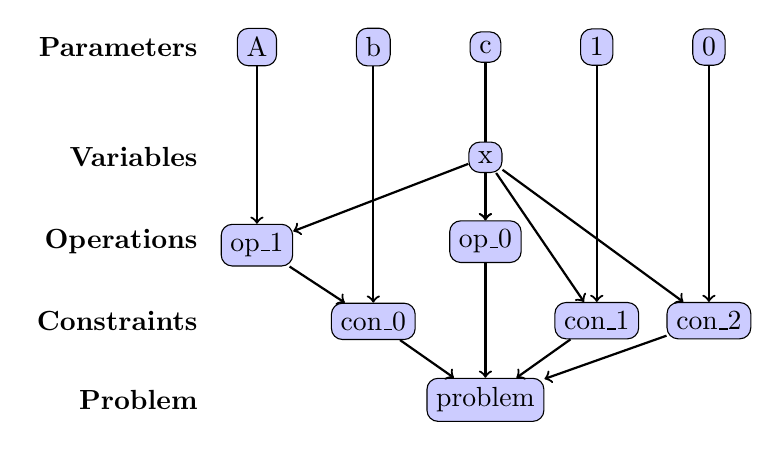
\begin{tikzpicture}[node distance=1cm]
        % Nodes
        % Parameters
        \node (A) [draw, rectangle, rounded corners, fill=blue!20, text centered] {A};
        \node (b) [right=of A, draw, rectangle, rounded corners, fill=blue!20, text centered] {b};
        \node (c) [right=of b, draw, rectangle, rounded corners, fill=blue!20, text centered] {c};
        \node (one) [right=of c, draw, rectangle, rounded corners, fill=blue!20, text centered] {1};
        \node (zero) [right=of one, draw, rectangle, rounded corners, fill=blue!20, text centered] {0};

        \node (op_0) [below=2cm of c, draw, rectangle, rounded corners, fill=blue!20, text centered] {op\_0};
        \node (op_1) [below=2cm of A, draw, rectangle, rounded corners, fill=blue!20, text centered] {op\_1};
        
        
        \node (con_0) [below=3cm of b, draw, rectangle, rounded corners, fill=blue!20, text centered] {con\_0};
        
        \node (con_1) [below=3cm of one, draw, rectangle, rounded corners, fill=blue!20, text centered] {con\_1};
        
        \node (con_2) [below=3cm of zero, draw, rectangle, rounded corners, fill=blue!20, text centered] {con\_2};
        \node (problem) [below=4cm of c, draw, rectangle, rounded corners, fill=blue!20, text centered] {problem};

        % Arrows
        \draw[->, thick] (A) -- (op_1);
        
        \draw[->, thick] (c) -- (op_0);
        
        \draw[->, thick] (op_1) -- (con_0);
        \draw[->, thick] (b) -- (con_0);
       
        \draw[->, thick] (one) -- (con_1);
        
        \draw[->, thick] (zero) -- (con_2);
        \draw[->, thick] (op_0) -- (problem);
        \draw[->, thick] (con_0) -- (problem);
        \draw[->, thick] (con_1) -- (problem);
        \draw[->, thick] (con_2) -- (problem);

        \node (x) [below=1cm of c, draw, rectangle, rounded corners, fill=blue!20, text centered] {x};
        \draw[->, thick] (x) -- (op_1);
        \draw[->, thick] (x) -- (op_0);
        \draw[->, thick] (x) -- (con_1);
        \draw[->, thick] (x) -- (con_2);

        % Add a common alignment anchor on the left
        \node (alignleft) [xshift=-0.25cm, anchor=east] at (A.west) {};

        % Parameters (aligned left)
        \node[anchor=east] at (alignleft |- A.center) {\textbf{Parameters}};
        
        % Variables (aligned left)
        \node[anchor=east] at (alignleft |- x.center) {\textbf{Variables}};
        
        % Operations (aligned left)
        \node[anchor=east] at (alignleft |- op_0.center) {\textbf{Operations}};
        
        % Constraints (aligned left)
        \node[anchor=east] at (alignleft |- con_0.center) {\textbf{Constraints}};
        
        % Problem (aligned left)
        \node[anchor=east] at (alignleft |- problem.center) {\textbf{Problem}};



    \end{tikzpicture}
    \caption{Directed computation graph demonstrating \texttt{Expression} relationships. The problem data in Code~\ref{lst:example_problem} is demonstrated as \texttt{Expressions} are linked together to create the \texttt{Problem}.}
    \label{fig:opt_problem}
\end{figure}


\subsection{LP Reductions}
\label{Reductions}
In order to solve a general linear programming (LP) problem using the simplex algorithm, the problem must first be transformed into a canonical form known as \emph{slack form}. The \texttt{Problem} class encapsulates this transformation process by reducing arbitrary LP input definitions into a set of structured matrix equalities and a standardized objective. This section outlines the full reduction pipeline used by the \texttt{to\_slack\_form} method.

An LP problem is provided as a dictionary with an objective function (\texttt{minimize} or \texttt{maximize}) and a list of constraints under \texttt{subject to} or \texttt{constraints}. Constraints may include inequalities, equalities, or non-negativity conditions.

The transformation to slack form proceeds through the following sequential reductions:

\begin{enumerate}
    \item \textbf{Bounded Variable Collection:} Non-negativity constraints are parsed to identify bounded variables (variables with $\geq 0$ restrictions). These are stored in \texttt{bounded\_vars}.
    
    \item \textbf{Non-negativity Stripping:} Non-negativity constraints are removed from the constraint list since they are tracked separately via variable flags.
        
    \item \textbf{Unbounded Variable Identification:} All variables appearing in the constraint set that were not previously identified as bounded are labeled as unbounded.
    
    \item \textbf{Equality Standardization:} Inequality constraints are transformed into equalities by introducing slack or surplus variables, which are appended to \texttt{bounded\_vars}.
    
    \item \textbf{Unbounded Variable Decomposition:} Every unbounded variable is replaced with a pair of non-negative variables $(x^+ - x^-)$, and a mapping is stored in \texttt{ub\_b\_map}.
    
    \item \textbf{Constraint Rewriting:} All existing constraints are rewritten in terms of the new bounded variable representations using the mapping.
    
    \item \textbf{Variable Indexing:} The final list of bounded variables is assigned a block index in the variable vector.
    
    \item \textbf{Variable Vector Creation:} All bounded variables are concatenated into a single flat vector \texttt{x\_big}, representing the problem’s variable space.
    
    \item \textbf{Matrix Formulation:} Each equality constraint is converted into a matrix row $(A_i, b_i)$ using \texttt{linear\_equality\_to\_matrix\_equality}, populating the matrices $A$ and $b$.

    \item \textbf{Constraint Concatenation:} Each $A_i$ and $b_i$ of each constraint is concatenated into one constraint with $A_{big}, b_{big}$ parameters.
    
    \item \textbf{Objective Vector Construction:} The objective function is linearized and mapped to a vector $c$ aligned with the same variable ordering.
    
    \item \textbf{Minimization Standardization:} If the problem is a maximization, it is converted to a minimization by negating the objective.
    \item \textbf{Solve: } The \texttt{two\_phase\_simplex} function is called and the problem solution is returned.
\end{enumerate}

\subsection{Final Form}

After the transformation, the problem is expressed in the canonical form:
\begin{align*}
\text{minimize} \quad & c^T x \\
\text{subject to} \quad & Ax = b \\
& x \geq 0
\end{align*}

Where $x$ is the flat vector \texttt{x\_big} composed of all bounded variables, including replacements for unbounded and slack variables. 
The vectors $c$, $b$ and matrix $A$ are stored in \texttt{c\_big}, \texttt{b\_big}, and \texttt{A\_big} respectively.

This slack form representation is then compatible with the two-phase simplex method and fed back in to the algorithm described previously in Algorithm~\ref{alg:two_phase_simplex}

\section{Results}
\label{sse:results}
\subsection{Testing}
The testing suite is available in the \texttt{tests.py} file.
In order to test the results of GatorPy, \textbf{CVXPY} is used as a comparison to ensure that GatorPy returns the correct solution.
The testing suite currently involves 7 simple LPs that are ran in both GatorPy and \textbf{CVXPY} and compared to each other.
GatorPy currently passes 6/7 unit tests, notably failing to drop auxiliary variables from the basis when the auxiliary variables outnumber the original set of variables.

Augmenting the testing suite with a richer set of LPs of varying sizes and problem structure is left as a next step in Section~\ref{sss:future_work}.
\subsection{GatorPy Usage}
To use GatorPy, proceed to the ECH4905 - Andres Espinosa repository GitHub link available in the references at \cite{repo:ech4905}.
The files for GatorPy are available at \texttt{project/gatorpy}.
Before attempting to run your own LP, ensure a Python version with NumPy.
This repository was only tested with Python=3.11 and NumPy=1.26.0.
The code is likely to work earlier/later versions but the code has not been verified to work with other versions.
To solve your own LP with GatorPy, download this folder, replace the example LP in \texttt{solve.py} with your own LP entered in the GatorPy modeling and finally run the \texttt{solve.py} file.

Publishing GatorPy as a standalone PyPi package available to install with \texttt{pip} is left as a next step in Section~\ref{sss:future_work}.

\section{Discussion}
\label{sse:discussion}
\subsection{Future Work}
\label{sss:future_work}
Several directions remain to enhance the solver's robustness, generality, and performance. 
Future efforts will focus on the following areas:

\begin{itemize}
    \item \textbf{Expanded Benchmarking Suite:} The current test suite could be augmented to include problems of varying sizes, particularly those with a large number of variables and constraints. 
    This would allow for a more thorough investigation of solver performance under computationally intensive scenarios.

    \item \textbf{Diverse Problem Structures:} The solver could be evaluated on a broader array of problem structures and formulations. 
    This would help assess the effectiveness and flexibility of the solver'’'s problem reduction mechanisms across different LP representations.

    \item \textbf{Extension to Mixed-Integer Programming (MIP):} Support for mixed-integer programs could easily be introduced by implementing a \texttt{BinaryVariable} object. 
    Algorithms such as branch-and-bound and Gomory cut methods could be incorporated to handle integrality constraints while still relying on the already implemented Simplex algorithm.

    \item \textbf{Extension to Convex Optimization:} A difficult, but rewarding extension could be to support general convex programs. 
    This involves introducing a set of \texttt{Function} objects representing common convex functions, which can be composed using disciplined convex programming (DCP) rules. 
    These enhancements would evolve the framework into a full-featured convex optimization solver.

    \item \textbf{Multiple Solver Algorithms:} Currently, the Simplex algorithm is the only algorithm available for running LPs through.
    This could be changed by defining a general \texttt{solver} structure that takes in a set of parameters and variables and outputs a solution.
    This would allow GatorPy to have multiple algorithms implemented such as interior-point methods.
    This would also be necessary in order to extend the solver to include convex problems, as the Simplex algorithm does not work with convex problems.

    \item \textbf{Efficient Language Switch:} Transitioning the solver's core implementation to a more efficient language such as Rust, Julia, or C++ could significantly improve performance, particularly for large-scale problems. 
    These languages offer better memory management and computational speed, making them ideal for optimization tasks.
\end{itemize}

\subsection{Conclusion}
GatorPy provides a clear, educationally focused implementation of a Linear Programming solver using pure Python and NumPy. 
By constructing a modular object-oriented framework and employing the two-phase Simplex method, GatorPy demystifies OR solvers and offers students an accessible entry point into optimization.

This project highlights how algorithmic transparency and thoughtful software design can enable a deeper understanding of optimization theory. 
From the algebraic modeling language to the step-by-step transformations into slack form, every component was engineered to maximize readability and reusability for future students. 
The solver successfully handles a range of LP problems, validates feasibility, and reliably computes optimal solutions, laying a solid foundation for future development.

However, there are many areas of improvement that this project could benefit from. 
Extensions to MIPs and Convex Programs is an interesting area of further work that could elevate GatorPy.
Rewriting the repository in another language could prove an incredibly rewarding challenge for learning both OR tools and another programming language.

Overall, GatorPy serves as both a functional solver and a pedagogical tool, offering a hands-on platform for students and practitioners to experiment with and better understand the mechanics of linear programming.

\clearpage
\section{Appendix}
\label{appendix}
% 1. Pivot Operation
\begin{algorithm}
    \caption{\texttt{pivot}}
    \label{alg:pivot}
    \begin{algorithmic}[1]
    \Require tableau $\textbf{T} \in \mathbb{R}^{m \times n}$, indices $r$ and $c$
    \Ensure tableau $\textbf{T}$
    \State $\textbf{T}_{r, :} \gets \textbf{T}_{r, :} / \textbf{T}{r, c}$ \Comment{normalize pivot row}
    \For{each row $i \neq r$}
        \State $\textbf{T}{i, :} \gets \textbf{T}{i, :} - \textbf{T}{i, c} \cdot \textbf{T}{r, :}$ \Comment{update rows}
    \EndFor
    \State \Return $\textbf{T}$ \Comment{return updated tableau}
    \end{algorithmic}
    \end{algorithm}
    
    % 2. Find Entering Variable
    \begin{algorithm}
    \caption{\texttt{find\_entering\_variable}}
    \label{alg:entering}
    \begin{algorithmic}[1]
    \Require tableau $\textbf{T} \in \mathbb{R}^{m \times n}$ 
    \Ensure index $j$, or None
    \For{$j = 1$ to $n - 1$}
        \If{$\textbf{T}_{m, j} < -\varepsilon$}
            \State \Return $j$ \Comment{return entering index}
        \EndIf
    \EndFor
    \State \Return none \Comment{no variables found}
    \end{algorithmic}
    \end{algorithm}
    
    % 3. Find Leaving Variable
    \begin{algorithm}
    \caption{\texttt{find\_leaving\_variable}}
    \label{alg:leaving}
    \begin{algorithmic}[1]
    \Require tableau $\textbf{T} \in \mathbb{R}^{m \times n}$, index $c$
    \Ensure index $r$, or None
    \State Initialize empty list $R$
    \For{$i = 1$ to $m - 1$}
        \If{$\textbf{T}_{i, c} > \varepsilon$}
            \State Append $(\textbf{T}_{i, n} / \textbf{T}_{i, c}, i)$ to $R$
        \EndIf
    \EndFor
    \If{$R$ is empty}
        \State \Return None \Comment{no variables found}
    \EndIf
    \State $r \gets \arg \min_R q$ \Comment{update row index}
    \State \Return $r$ \Comment{return leaving index}
    \end{algorithmic}
    \end{algorithm}
    
    % 4. Simplex Phase 1
    \begin{algorithm}
    \caption{\texttt{simplex\_phase\_1}}
    \label{alg:phase1}
    \begin{algorithmic}[1]
    \Require Matrix $\textbf{A}$, vector $\textbf{b}$
    \Ensure  Matrix $\textbf{A}$, vector $\textbf{b}$, list $B$, or None
    \State $\textbf{A}_{aux} := [\textbf{A} \; \textbf{I}]$
    \State \textbf{T} := 
    $\begin{bmatrix}
    \textbf{A} & \textbf{I} & \textbf{b} \\
    -\mathbf{1}^\top \textbf{A} & -\mathbf{1}^\top & -\mathbf{1}^\top \textbf{b}
    \end{bmatrix}$
    \State $B := [\text{dim}(\textbf{A})_2,\dots,\text{dim}(\textbf{A}_{aux})_2]$
    \While{true}
        \State $c \gets $ \texttt{find\_entering\_variable}$(\textbf{T})$
        \If{$c$ is None}
            \State \textbf{break}
        \EndIf
        \State  $r \gets $ \texttt{find\_leaving\_variable}$(\textbf{T},c)$
        \If{none found}
            \State \Return None \Comment{return infeasible}
        \EndIf
        \State $\textbf{T} \gets $ \texttt{pivot}($\textbf{T},c,r$)
    \EndWhile
    \If{$T_{-1,-1}$ $> 0$} \Comment{positive objective value}
        \State \Return None \Comment{return infeasible}
    \EndIf
    \State $\textbf{T} \gets $ \texttt{pivot}($\textbf{T},c,r$) \Comment{remove aux vars}
    \State $\textbf{A}, \textbf{b} \gets \textbf{T}$
    \State \Return $A$, $b$, $B$
    \end{algorithmic}
    \end{algorithm}
    
    % 5. Simplex Phase 2
    \begin{algorithm}
        \caption{\texttt{simplex\_phase\_2}}
        \label{alg:phase2}
        \begin{algorithmic}[1]
        \Require Matrix $\textbf{A}$, vector $\textbf{b}$, cost vector $\textbf{c}$, basis $B$
        \Ensure Optimal value $f^*$, solution $\textbf{x}^*$, or Unbounded
        \State $\textbf{T} := \begin{bmatrix} \textbf{A} & \textbf{b} \\ -\textbf{c}^\top & 0 \end{bmatrix}$
        \State Adjust cost row from $B$ 
        \While{true}
            \State $c \gets$ \texttt{find\_entering\_variable}($\textbf{T}$)
            \If{$c$ is None}
                \State \textbf{break} \Comment{optimality reached}
            \EndIf
            \State $r \gets$ \texttt{find\_leaving\_variable}($\textbf{T}, c$)
            \If{$r$ is None}
                \State \Return \texttt{Unbounded}
            \EndIf
            \State $\textbf{T} \gets$ \texttt{pivot}($\textbf{T}, r, c$)
            \State Update basis $B$ with $B[r] \gets c$
        \EndWhile
        \State Extract solution $\textbf{x}^*$ from $\textbf{T}$ using basis $B$
        \State $f^* \gets -\textbf{T}_{-1, -1}$ \Comment{optimal value from cost row}
        \State \Return $f^*$, $\textbf{x}^*$, feasible = true
        \end{algorithmic}
    \end{algorithm}


\bibliographystyle{IEEEtran}
\bibliography{references}  % Assuming your .bib file is named references.bib


\end{document}



